\chapter{Modulo configurazione prodotto}\label{chapter:Configurazione}
\section{Scopo del modulo}
Il vero salto di qualità, rispetto all'attuale metodo di creazione delle offerte,
è l'introduzione di un modulo di configurazione prodotto.
Come ciatto nell'introsuzione\ref{chapter:introduction}, l'azienda ha un modello di bussiness
di tipo \ac{ETO}. QUesto modello comporta la produzione di prodotti cuciti
su misura per il ciente, utilizzando però compoennti stadardizzati.
Si è docuto quindi cercare di realizzare una struttura ed un algoritmo che permettesse 
di configurare un prodotto, senza sapere a priori nè da quali regole sia governato nè quali prodotti.
è stato fondamentale anche lo studio di un sistema che guidasse l'utente alla scelta del modello da configurare.
\section{Algoritmo di configurazione}
L'algoritmo implementato si suddivide in tre fasi principali:
\begin{itemize}
    \item \textbf{Fase di scelta del modello:} Mediante una scelta
    a castata l'utente discende da concetti generali come scopo del compoenente alla tipologia di prodotto,
     fino ad arrivare al modello specifico da configurare.
     Questo modella ad albero guida l'utente.
    \item \textbf{Fase di configurazione:} In questa fase vengono proposti all'utente delle
    opzioni di configurazione per il modello scelto.
    \item \textbf{Fase scelta componenti:} In base alle scelte prima
    all'utente vengono proposti i componenti disponibili per la configurazione del prodotto.
    Di questi è posibile in questa fase eliminare quelli non desiderati.
    \item \textbf{Generazione codice:} Questa fase 
    finale è la delicata dell'implementazione dell'algoritmo, in quanto in base ai codici scelti si hanno
    due alternativi:
    \begin{itemize}
        \item \textbf{Configurazione esistente:} Si ricerca nel database se esiste già una configurazione
        di quel prodotto con i codici scelti.
         In caso positivo si propone all'utente di utilizzare quella configurazione.
        \item \textbf{Configurazione inesistente:} In caso negativo, 
        si genera un nuovo codice di configurazione per il prodotto, che viene salvato nel database.
    \end{itemize}
\end{itemize}
\subsection{Scelta macrogruppo da configurare}
La realizzazione dell'albero di scelta è stata fatta sfruttando
le tabelle già presenti nel database, in particolare le tabelle prodotto, prodotti\_composizioni e di lookup.
Si sono atribuiti tre nuovi tipi di prodotto ovvero: iniziale, mappa e macrogruppo.
Il prodotto iniziale è la radice dell'albero, e rappresenta il concetto generale del prodotto.
Si sono inseriti all'interno delle loro distinte i prodotti di tipo mappa, che rappresentano i concetti intermedi.
Infine i prodotti di tipo macrogruppo rappresentano i prodotti finali, sono stati a loro volta inseriti
 nelle distinte dei prodotti di tipo mappa.
 Questa struttura permette la realizazione di un albero ampliamente scalabile,
  in quanto è possibile aggiungere nuovi prodotti senza dover modificare l'algoritmo.
L'albero in questione è osservabile in figura~\ref{fig:Albero di scelta prodotto}.
\begin{figure}[H]
    \centering
    \includegraphics[width=0.6\linewidth]{figures/AlberoScelta.png}
    \caption{Albero di scelta prodotto}\label{fig:Albero di scelta prodotto}
\end{figure}
\subsection{Implentazione regole}
I macrogruppi contengono al loro interno tutti i componenti possibili per la configurazione del prodotto.
Ad ogni componente sono state associate n regole che, se valide, determinano la sua disponibilità nella configurazione.
Ad ogni regola a sua volta è associata una proprità di riferimento, un operatore logico e un valore di riferimento.
L'interfaccia utente con le possibili domande di configurazione
viene generata filtrando dinamicamente tutte le proprietà di riferimento delle regole, in base al macrogruppo scelto.
In questo modo non si ha la necessità di conoscere a priori le regole che governano la configurazione del prodotto.
In base alle scelte, come detto in precedenza, si propongono all'utente solo i componenti che rispettano le scelte effettuate.
La realizzazione lato database è stata possibie introducendo due 
nuove tabelle, una per le regole ed una di lookup per gli operatori logici.
La struttura dinamica del database, impletata nelle prime fasi, ha permesso l'implementazione in modo agile.
Di seguito nella figura~\ref{fig:ER configuratore} è possibile il modello \ac{ER} del modulo di configurazione prodotto.
\begin{figure}[H]
    \centering
    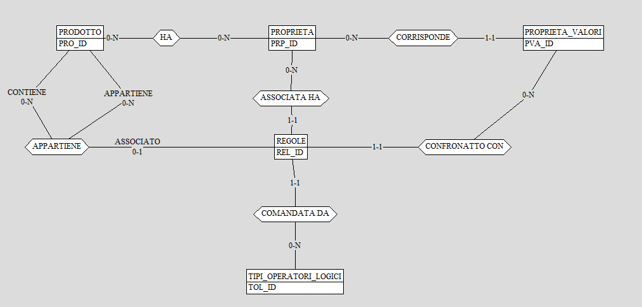
\includegraphics[width=0.6\linewidth]{figures/ER_Configuratore.png}
    \caption{Modello ER configuratore}\label{fig:ER configuratore}
\end{figure}
\section{Interfaccia grafica lato utente ed amministratore}
Le intefacce lato utente ed amministratore sono profondamente diverse, in quanto per dare 
all'untente una esperienza di configurazione semplice e guidata, 
la complessità è stata spostata lato amministratore.
\subsection{Lato utente}
L'esperienza di configurazione lato uetnte è stata realizzato dopo
un focus group con alcuni utenti, in cui si è cercato di capire quale potesse essere
il flusso di lavoro più semplice e intuitivo.
Si è deciso di proporre le scelte successive solo dopo aver effettuato la scelta precedente,
 in modo da guidare l'utente.
 Si è partito dai concetti generali, come lo scopo del prodotto, fino ad arrivare al modello specifico da configurare.
 Nella figura~\ref{fig:Interfaccia lato utente} è possibile osservare l'interfaccia grafica lato utente.
 \begin{figure}[H]
    \centering
    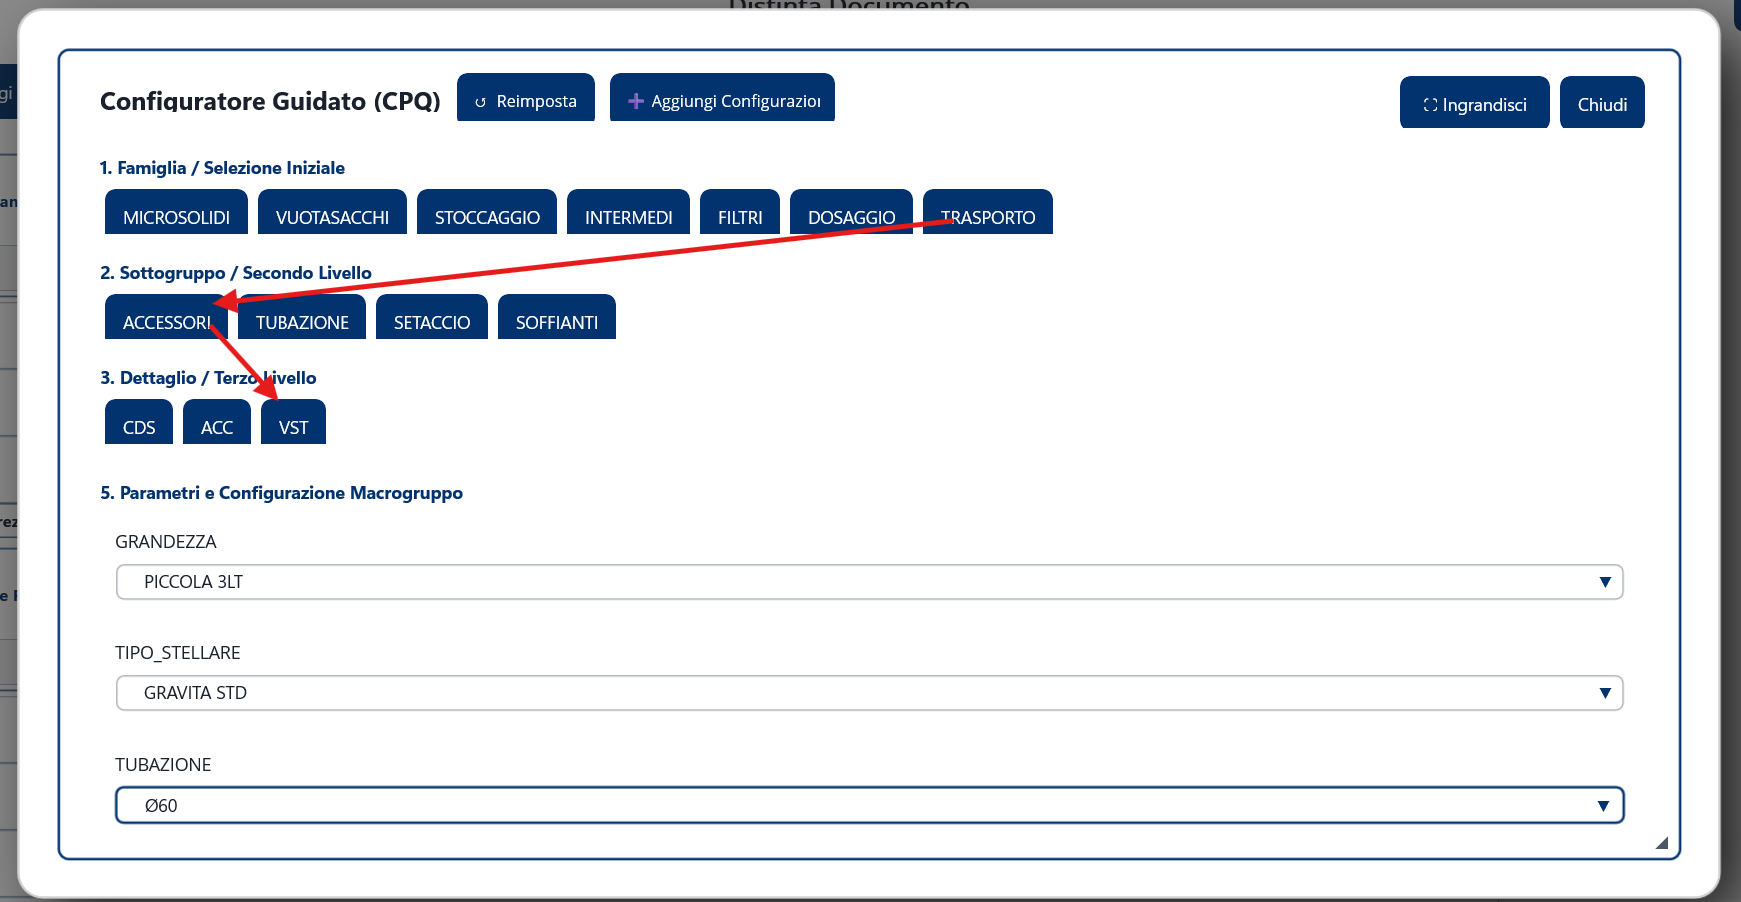
\includegraphics[width=0.6\linewidth]{figures/ConfigurazioneLatoUtente.png}
    \caption{Configurazione lato utente}\label{fig:Configurazione lato utente}
 \end{figure}
 Il risultato finale è visibile nella figura~\ref{fig:Risultato configurazione lato utente} sottostante.
  \begin{figure}[H]
    \centering
    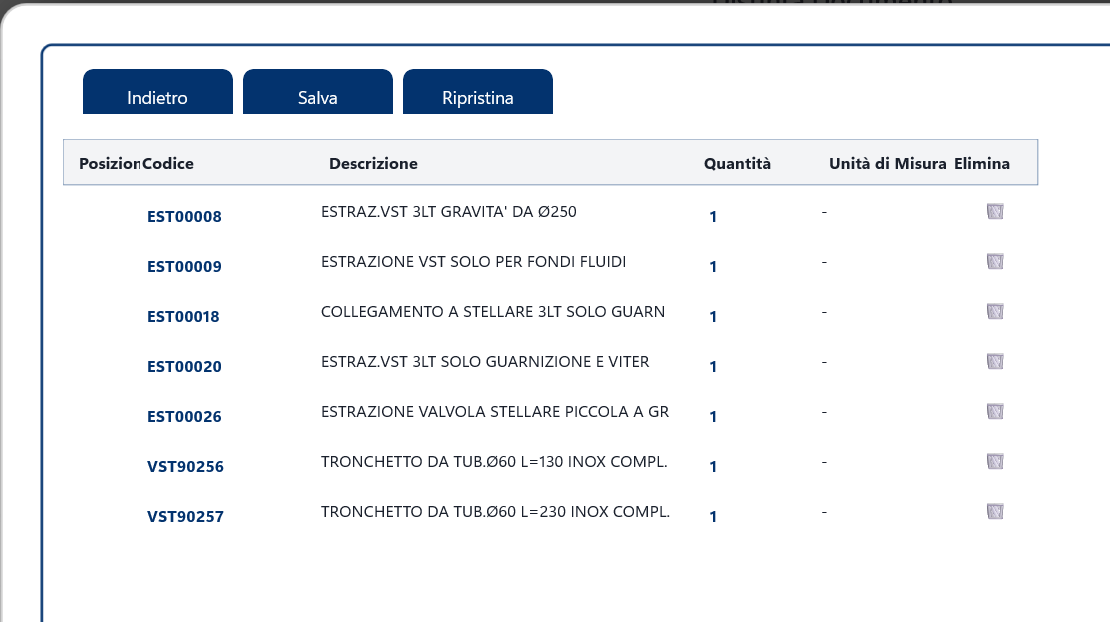
\includegraphics[width=0.6\linewidth]{figures/RisultatoConfigurazione.png}
    \caption{Risultato configurazione lato utente}\label{fig:Risultato configurazione lato utente}
 \end{figure}
 Al termine il codice generato o raccolto dal database viene aggiunto ai prodotti dell'offerta,
  e l'utente può proseguire con la creazione dell'offerta.
\subsection{Lato amministratore}
La creazione delle configurazioni passa dalla composizione dei macrogruppi.
Dopo aver compilato con i compoenenti, a questo punto ad ognuno di essi possono venire assegnate una o più
regole.
L'assegnazione avviene aggiungenedo la proprietà di riferimento, l'operatore logico e il valore che deve
 essere rispettato per rendere disponibile il componente.
 Di seguito l'interfaccia di aggiunta delle regole ad un componente,
  visibile in figura~\ref{fig:Interfaccia lato amministratore}.
  Si può notare a detra la scelta delle proprietà mediante filtri, e a sinistra la lista delle
  regole già assegnate al componente.
  \begin{figure}[H]
    \centering
    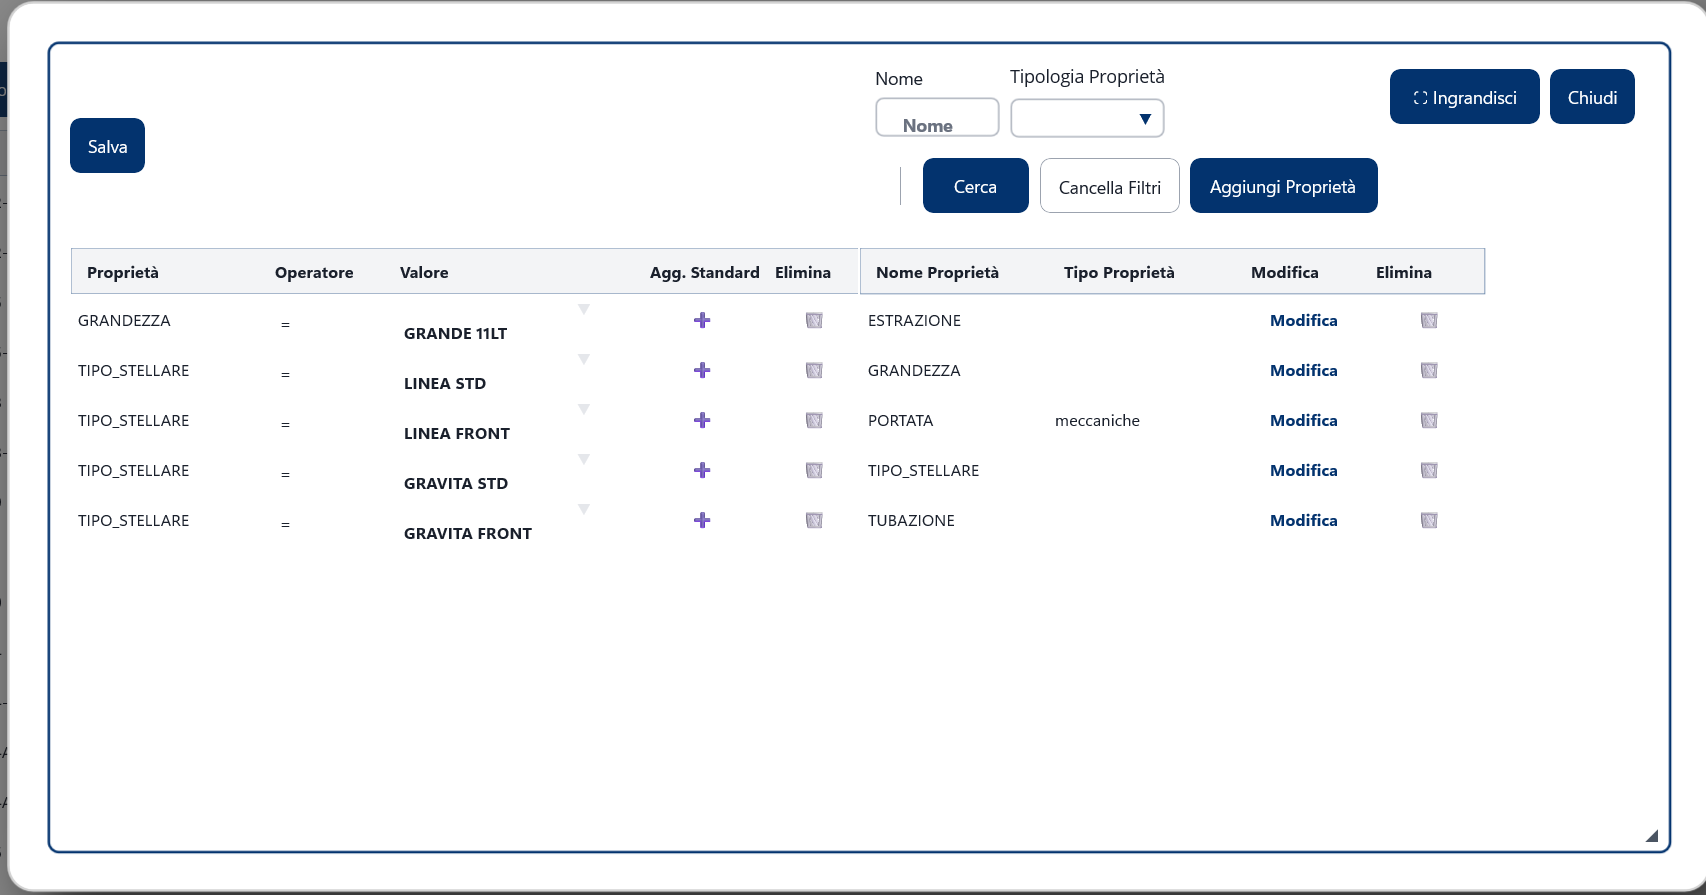
\includegraphics[width=0.9\linewidth]{figures/AggiuntaRegole.png}
    \caption{Aggiunta regole}\label{fig:Aggiunta regole lato amministratore}
  \end{figure}
  Dal focus gruop con gli utenti che potrebbero gestire la crezione è emerso come
  il testare le regole sia un aspetto fondamentale, in quanto permette di capire se le regole inserite
  sono corrette e se il flusso di configurazione è coerente.
  Si è quindi creata un'interfaccia di test delle regole, visibile in figura~\ref{fig:Test regole lato amministratore}.
  \begin{figure}[H]
    \centering
    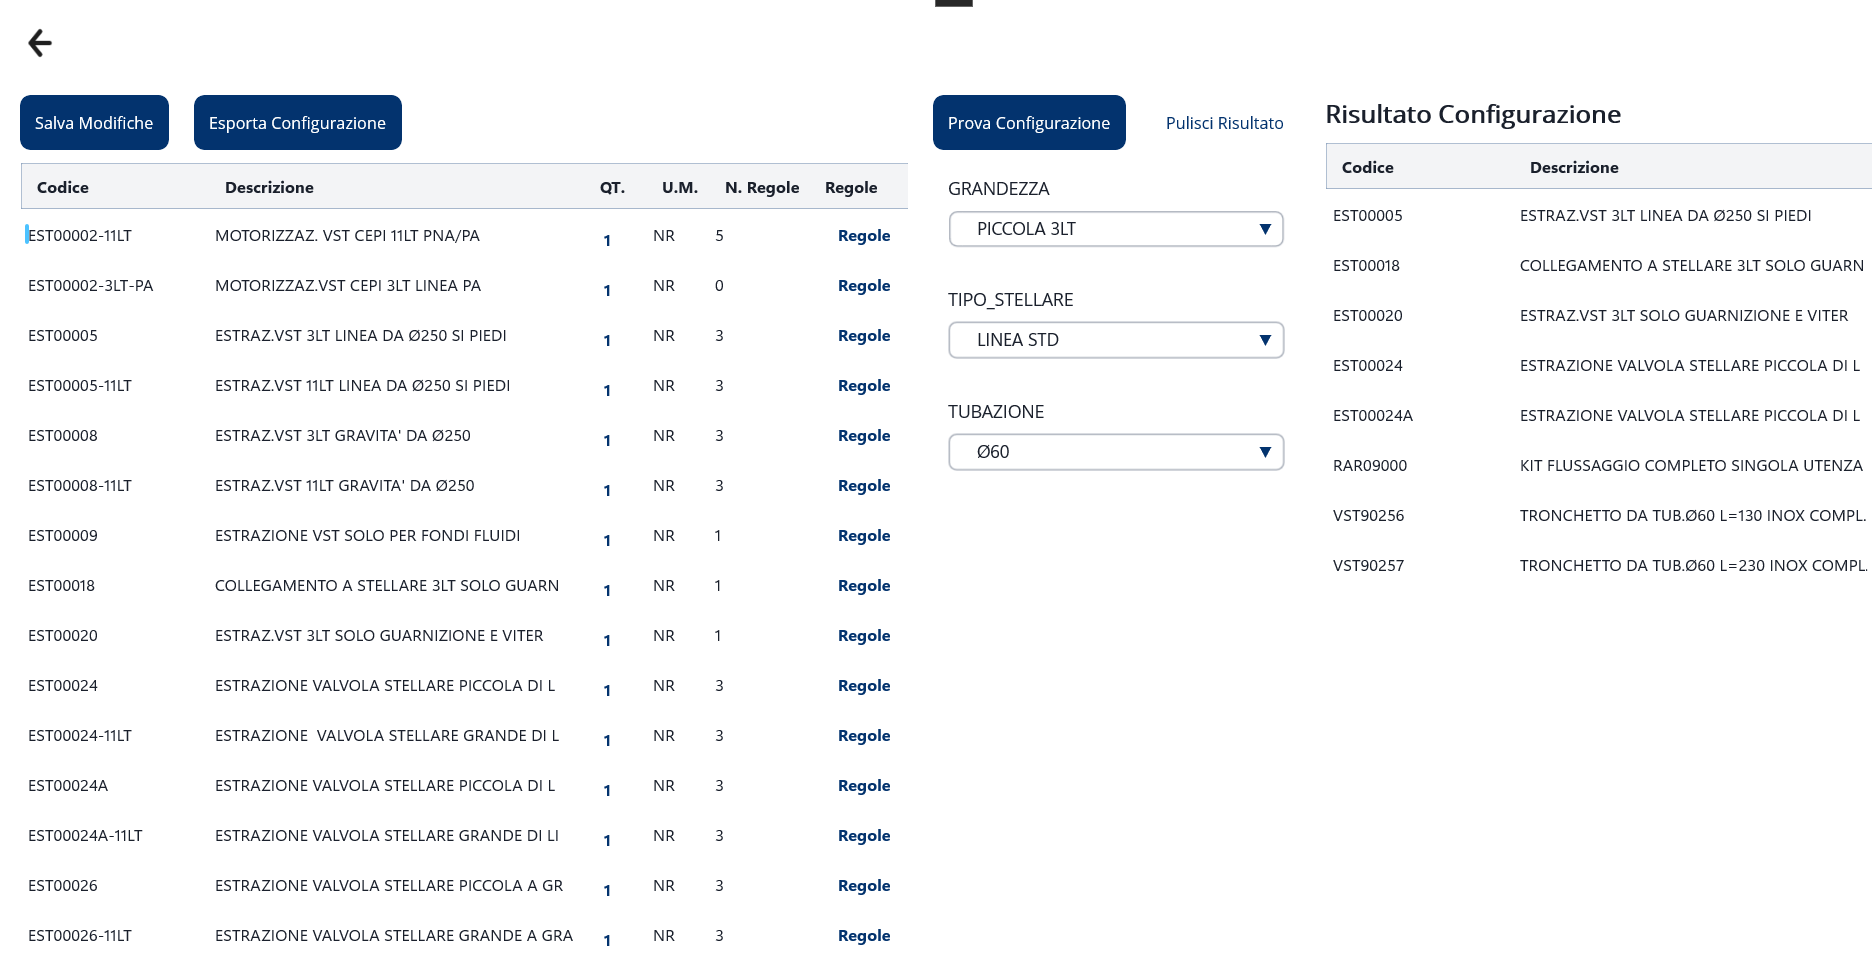
\includegraphics[width=0.9\linewidth]{figures/TestConfigurazione.png}
    \caption{Test regole lato amministratore}\label{fig:Test regole lato amministratore}
    \end{figure}